\documentclass[a7paper,print]{kartei}
\usetikzlibrary{positioning,calc}

\usepackage[utf8]{inputenc}
\usepackage[ngerman]{babel}
\def\miss{\textcolor{red}{Missing answer}}
\def\oo{objektorientiert}
\def\Oo{Objektorientiert}
\usepackage{paralist}
\usepackage{tikz,tikz-uml}
\usepackage{amsmath}
\usepackage{amssymb}

\newcommand{\card}[2]{
\begin{karte}[SEng]{#1}
	\scriptsize #2
\end{karte}
}

\begin{document}

\card{Was ist ein \textbf{fault}?}{
	Fehler, der von Menschenhand während der Laufzeit der Software getätigt wurde (fehlerhaftes Design, Anforderungen, Coding)\\
	(Anschalten der Kühlung (Atomkraftwerk) nicht korrekt programmiert)
}

\card{Was ist ein \textbf{failure}?}{
	Ein Fehler in der gelieferten Software, die nicht mehr ihren Spezifikationen entspricht (nicht mehr das tut, was zu erwarten wäre).\\
	Bzw.: Die Unfähigkeit eines Systems oder einer Komponente seine geforderten Funktionen innerhalb der Leistungsanforderungen durchzuführen.\\
	(Atomkraftwerk explodiert)
}

\card{Charakteristik von technischer Disziplin (Engineering Discipline)}{
	\begin{enumerate}
		\item gut verstandene Technologien
		\item gut definierte Prozesse
		\item Vorhersagbarkeit eines Ergebnisses eines Prozessstils
		\item Wiederholbarkeit von Prozessschritten
	\end{enumerate}
}

\card{Welche Symptome traten in der Softwarekrise auf?}{
	\begin{enumerate}
		\item Produkte wurden zu spät geliefert (hohe Kosten)
		\item Projekte überschritten ihr Budget (hohe Kosten, Verschwendung von Ressourcen)
		\item Produkte taten nicht das, was sie tun sollten/wozu sie entwickelt wurden (ineffizient, hohe Kosten)
		\item Produkte waren defekt (hohe Kosten (failure, Wartung), ethische Überlegungen)
		\item Projekte wurden beendet, bevor sie abgeschlossen waren (Verschwendung von Ressourcen)
	\end{enumerate}
}

\card{Charakteristik von Software}{
	\begin{enumerate}
		\item Software wird entwickelt nicht hergestellt
		\item Software leiert nicht aus (aber: Veränderung von Anforderungen oder der Umwelt)
		\item Software ist komplex
		\item Software ist ein bestimmender Systemfaktor (bis zu 80\% des Entwicklungsaufwandes)
	\end{enumerate}
}

\card{Warum ist Software schwierig zu entwickeln?}{
	\begin{enumerate}
		\item es gibt kein ähnliches System bisher (Probleme sind unbekannt, Annahmen zur Umgebung können falsch sein)
		\item Anforderungen sind nicht gut/ausreichend verstanden/formuliert
		\item Anforderungen verändern sich im Laufe der Entwicklung des Systems
		\item komplexe Interaktion
		\item Natur des Systems: nebenläufige Systeme (Deadlocks, \dots), eingebettete Systeme (Hardwareinteraktion, Timing, \dots), Informationssysteme (Komplexität, \dots)
		\item Software ist einfach zu verändern ("`code and fix"')
		\item Software ist unauffällig (entweder fällt sie aus, oder nicht)
	\end{enumerate}
}

\card{Software-Entwicklungs-Mythen}{
	\begin{enumerate}
		\item Management:\\
			- Standard-Bücher, -Software, -Tools $\Rightarrow$ Software ist schwierig zu standardisieren\\
			- Dem Zeitplan hinterher? Programmieren einstellen $\Rightarrow$ Bemühung neue Leute einzustellen
		\item Kunde:\\
			- allgemeine Erklärung der Ziele sind ausreichend\\
			- Veränderungen (auch in den Anforderungen) sind einfach zu implementieren
		\item Anwender:\\
			- Sobald das Programm läuft ist der Job erledigt\\
			- Bis das Programm läuft gibt es keine Möglichkeit die Qualität des Systems zu überprüfen\\
			- Nur ein arbeitsfähiges Programm ist lieferbar
	\end{enumerate}
}

\card{Was ist Software Engineering?}{
	\begin{enumerate}
	\item Kommunikation zwischen einer großen Anzahl von Parteien (Kunde, Endbenutzer, Software Designer, Entwickler, \dots) wird aufrechterhalten
	\item Die Basis der Softwareproduktion ist der Entwicklungsansatz.
	\item Design der Software als Prozess, der folgendes unterstützt:
		\begin{enumerate}
			\item Korrektheit und Zuverlässigkeit
			\item Kosteneffizienz
			\item Komplexität des Projektes
			\item Langlebigkeit des Produktes, Lebenszyklus, Veränderungen
			\item Kommunikation unter den Parteien
		\end{enumerate}
	\end{enumerate}
}

\card{Definition des Software Engineering Prozessmodelles}{
	alle Phasen des Software Engineeringprozesses: strikte Anwendung des Prozessmodells (wohldefinierter Input/Output)
}

\card{Built-and-Fix-Modell}{
	\begin{enumerate}
		\item keine Prozessschritte
		\item keine Unterteilung von Bedenken
		\item keine Möglichkeit mit Komplexität umzugehen
	\end{enumerate}
	\usetikzlibrary{positioning,arrows}
\begin{tikzpicture}[every node/.style={draw,rounded corners,text width=1.8cm},node distance=0.5cm, dev/.style={->,>=triangle 60},main/.style={dev,dashed}]
\node (0) at (0,0) {Build first version};
\node (1) [right=of 0] {Modify until client is satisfied};
\node (2) [below right=of 1] {Operations Mode};
\node (3) [above right=of 2] {Retirement};
\node (p1) [above=of 0,draw=none] {\ };
\node (p2) [right=of 1,draw=none,xshift=-1cm,yshift=-0.2cm] {\ };
\node (p3) [below=of 1,draw=none,yshift=0.4cm,xshift=0.3cm] {\ };

\path[dev,draw](0)--(p1.center)-|(1);
\path[dev,draw](1)|-(2);
\path[dev,draw](1)to[out=300,in=90](p3.center)-| (p2.center)to[out=180,in=-10](1);
\path[main,draw](2)|-(1);
\path[dev,draw](2)-|(3);

\draw[->,>=triangle 60] (-1,-2)--(1,-2);
\draw[->,>=triangle 60,dashed] (-1,-2.5)--(1,-2.5);
\node (dev)[anchor=west,draw=none] at (1.2,-2) {Development};
\node (main)[anchor=west,draw=none] at (1.2,-2.5) {Maintenance};
\end{tikzpicture}
}
\card{Wasserfall-Modell (Bild)}{
	\usetikzlibrary{positioning}

\begin{tikzpicture}[every node/.style={draw, fill=black!10}, node distance=0.6cm]

\node(0) at(0,0) {System Design};
\node(1)[below=of 0,anchor=north west]{Requirements};
\node(2)[below=of 1,anchor=north west]{Design};
\node(3)[below=of 2,anchor=north west]{Implementation};
\node(4)[below=of 3,anchor=north west]{Integration};
\node(5)[below=of 4,anchor=north west]{Maintenance};

\foreach \x/\y/\z in {0/1/\ ,1/2/SRS,2/3/Design,3/4/Test,4/5/Test}{
	\draw[->](\x.east)to[out=0,in=20]node[right, draw=none,fill=none]{\scriptsize \z}(\y);
}

\foreach \x/\y/\z in {0/1/what ,1/2/how,2/3/\ ,3/4/\ ,4/5/\ }{
	\draw[->,dotted,color=red](\y)to[out=180,in=240]node[left, draw=none,fill=none]{\scriptsize \z}(\x);
}


\end{tikzpicture}
}

\card{WasserFall-Modell: System Design}{
	Probleme und Systemanforderungen, Realisierbarkeitsstudie, Definieren von Haupt-Subsystemen (zugeordnet zu Hard-/Software), System Design Document (SDD, informell, mit dem Kunden, manchmal: Bedienungsanleitungen, Benutzerschnittstellen, Testpläne)
}

\card{Wasserfall-Modell: Requirements}{
	Anforderungsanalyse ("`Was"' soll das System tun (nicht "`wie"'), Softwareanforderungen beschreiben die beobachtbaren externen Verhalten (funktional, non-funktional)), Software Requirement Specification (SRS)
}

\card{Wasserfall-Modell: Design}{
	"`Wie"' das System arbeitet, architektonisches (high level) Design (zerteilt das Problem in Komponenten, globale Datenstrukturen, interne Schnittstellen), detailliertes Design (algorithmisches Design, interne Datenstrukturen, Programmiersprache(n))
}

\card{Wasserfall-Modell: Implementation (und Testing)}{
	Übersetzung der Designmodule in Code, Testen der Module in Isolation
}

\card{Wasserfall-Modell: Integration (und Testing)}{
	Integrieren der getesteten Module zur Bildung des Systems, \textit{integration testing}, Bestätigung (Validation), Kundenakzeptanztests
}

\card{Wasserfall-Modell: Maintenance (Instandhaltung)}{
	Produktbereitstellung, Wartungsarbeiten (korrekt, adaptiv, perfekt), Projekt abschließen
}

\card{Wasserfall-Modell: Vorteile}{
	\begin{enumerate}
		\item \textbf{Dijkstra}: Definition der einzelnen Aufgaben, (Aufteilung der Bedenken) \\
			Aufteilen von komplexen Designproblemen in kleinere Einheiten $\Rightarrow$ vereinfacht die Teamarbeit/Reproduzierbarkeit
		\item Spezifikation und Dokumentation $\Rightarrow$ erzwingt Dokumentation, vereinfacht das Testen (entgegen der Anforderungsspezifikation)
		\item weitere Konzepte:
			\begin{enumerate}
				\item Verifikation/Validierung (Vergleicht Zwischenergebnisse von Anforderungen und Design)
				\item Prototyping (mock-up (Modell) ist früh verfügbar, reduziert Risiken)
				\item evolutionäres Prozessmodell (Unterbringen von Veränderungen)
			\end{enumerate}
	\end{enumerate}
}

\card{Wasserfall-Modell: Mängel}{
	\begin{enumerate}
		\item keine Rückkopplungsschleifen
		\item dokumentorientiert, unflexibel
		\item großer Zeitabstand zwischen Beginn und Abschluss
	\end{enumerate}
}

\card{Wasserfall-Modell: Alternativen}{
	\begin{enumerate}
		\item modifiziertes Wasserfallmodell
		\item V-Modell, V-Modell XT
		\item evolutionäre Prozess-Modelle
		\item Spiralmodell
		\item Rational Unified Process (RUP)
		\item Agile Prozesse
		\item \dots
	\end{enumerate}
}

\card{V-Modell: Bild}{
	\hspace*{-0.5cm}
	\scalebox{0.75}{\usetikzlibrary{positioning,calc,arrows}

\begin{tikzpicture}[every node/.style={draw,fill=white}, node distance=0.6cm]

\node(1) at (0,0)[anchor=north west,xshift=-.5cm]{Requirements Analysis};
\node(2)[below=of 1,anchor=north west,xshift=-0.25cm]{System Design};
\node(3)[below=of 2,anchor=north west,xshift=-0.15cm]{Program Design};
\node(4)[below right=of 3,anchor=north west,xshift=-0.25cm]{Coding};

\node(31)[right=of 3,anchor=west,xshift=0.6cm]{Unit and Integration Testing};
\node(21)[above=of 31,anchor=south west,xshift=-.6cm]{System Testing};
\node(11)[above=of 21,anchor=south west,xshift=-1cm]{Acceptance Testing};
\node(01)[above=of 11,xshift=.5cm] {Operation and Maintenance};

\foreach \x in {1,2,3}{
	\draw[->, dashed, >=triangle 60](\x1.west)to (\x.east);
}
\foreach \x/\y in {1/2,2/3,3/4}{
	\draw[->, >=triangle 60](\x)-- (\y);
}
\foreach \x/\y in {31/21,21/11,11/01}{
	\draw[->, >=triangle 60](\x.north)-- (\y.south);
}
\draw[->, >=triangle 60](4.east)-- (31.south);
\end{tikzpicture}}
}
\card{Software Qualitäten}{
	\begin{enumerate}
		\item Korrektheit
		\item Zuverlässigkeit
		\item Robustheit
		\item Wartbarkeit
		\item Performance
		\item Wiederverwendbarkeit
		\item Kompatibilität
	\end{enumerate}
}
\card{Software Qualitäten: Korrektheit}{
	die Software verhält sich entsprechende der Anforderungsspezifikation
}
\card{Software Qualitäten: Zuverlässigkeit}{
	die Software garantiert eine gewisses Level an Qualität (siehe Korrektheit)
}
\card{Software Qualitäten: Robustheit}{
	die Software verhält sich auch "`vernünftig"' in unerwarteten Umständen (Eingang, Stromausfall, \dots)
}
\card{Software Qualitäten: Wartbarkeit}{
	die Software ist einfach aufrechtzuerhalten und zu erweitern
}
\card{Software Qualitäten: Performance}{
	das System ist benutzbar (z.B. Eingangsreaktionszeit)
}
\card{Software Qualitäten: Wiederverwendbarkeit}{
	Wiederverwendbarkeit von zuvor Verwendetem, getesteter und geprüfter Code
}
\card{Software Qualitäten: Kombatibilität}{
	Standarisierung, Schnittstellen, \dots
}
\card{Softwareentwicklungsprinzipien}{
	\begin{enumerate}
		\item Strenge
		\item Formalität
		\item Trennung von Bedenken
		\item Abstraktion
		\item Modularität
		\item Allgemeinheit
	\end{enumerate}
}

\card{Softwareentwicklungsprinzipien: Strenge}{
	benutzen einer Methode und konsequent anwenden auf jeden Schritt
}
\card{Softwareentwicklungsprinzipien: Formalität}{
	benutzen von (mathematischen) formalisierbaren Methoden und Notationen
}
\card{Softwareentwicklungsprinzipien: Trennung von Bedenken}{
	sich mit verschiedenen Aspekten in separaten Schritten befassen
}
\card{Softwareentwicklungsprinzipien: Abstraktion}{
	trennen der Anliegen der wichtigen Aspekte von den Anliegen der unwichtigen Aspekte
}
\card{Softwareentwicklungsprinzipien: Modularität}{
	zerteilen des Problems in unabhängige Module (siehe Trennung von Bedenken)
}
\card{Softwareentwicklungsprinzipien: Allgemeinheit}{
	konzentrieren auf die Entdeckung von generellen Problemen
}
\card{Was sind Anforderungen?}{
	\begin{enumerate}
		\item "`A requirement is a condition or capability that must be met or professed by a system component to satisfy a contract, standard, specification or other formally imposed document."' (ANSI/IEEE Standad 729-1983)\\
		Eine Anforderung ist eine Bedingung oder Fähigkeit, die eine Systemkomponente erfüllen muss um einen Vertrag, einen Standard, eine Spezifikation oder eine anderes formales, verlangtes Dokument zu erfüllen/befriedigen.
		\item Anforderungen sind eine Beschreibung der von außen sichtbaren Verhalten, das "`was"'
		\item Anforderungen sind Interaktionen zwischen dem System und dem systemrelevanten Teil der Umwelt
	\end{enumerate}
}

\card{Benutzer- (Auftraggeber-) Anforderungen}{
	Aussagen in natürlicher Sprache mit Diagrammen
}

\card{Systemanforderungen}{
	strukturiertes Dokument, detaillierte Beschreibung der Systemfunktionen, Dienstleistungen und optionalen Einschränkungen; kann Teil des Vertrages zwischen Auftraggeber und Auftragnehmer
}

\card{Typen von Anforderungen}{
	\begin{enumerate}
		\item funktionale
		\item nicht-funktionale
			\begin{enumerate}
				\item Produktanforderungen
				\item Unternehmensanforderungen
				\item externe Anforderungen
			\end{enumerate}
		\item Domainanforderungen
	\end{enumerate}
}

\card{funktionale Anforderungen}{
	\begin{compactenum}
		\item high-level "`was"' das System tut, nicht wie
		\item Aussage darüber, welche Services das System anbieten sollte
		\item Interaktion zwischen System und Umwelt (Systemzustände, I/O)
		\item wie sich das System in besonderen Situationen verhalten sollte
		\item beschreibt den Service des System im Detail
		\item oft beschrieben mit soll/sollte
		\item "`funktionale Anforderungen legen fest, welche Dienste (aus Sicht des Benutzers) das System anbieten soll/welche Aufgaben es erfüllen soll
		\item eindeutig/widerspruchsfrei
		\item zentrale Vorgaben für die Systementwicklung
		\item beschrieben mit Use-Cases
	\end{compactenum}
}

\card{nicht-funktionale Anforderungen: Diagramm}{
	\usetikzlibrary{trees}

\begin{tikzpicture}[
  g/.style={rectangle,draw,fill=green!20,rounded corners=.8ex},
  yel/.style={rectangle,draw,fill=yellow!20,rounded corners=.8ex},
  gr/.style={rectangle,draw,fill=black!10,rounded corners=.8ex},
  b/.style={rectangle,draw,fill=blue!20,rounded corners=.8ex},
  grandchild/.style={grow=down,xshift=1em,anchor=west,
    edge from parent path={(\tikzparentnode.south) |- (\tikzchildnode.west)}},
 ggrandchild/.style={grow=right,xshift=1em,anchor=west,
    edge from parent path={(\tikzparentnode.east) |- (\tikzchildnode.west)}},
  first/.style={level distance=4.5ex},
  second/.style={level distance=9ex},
  third/.style={level distance=13.5ex},
  fourth/.style={level distance=18ex},
  level 1/.style={sibling distance=5em}]
    % Parents
    \coordinate
      child[grow=down,level distance=0ex]{node[b, anchor=west]{nicht-funktional}}
    [edge from parent fork down]
    % Children and grandchildren
    child{node[g,xshift=-1.3cm] {produktspezifische}
      child[grandchild,first] {node[yel]{Nutzbarkeit}}
      child[grandchild,second] {node[yel]{Realisierbarkeit}}
      child[grandchild,third] {node[yel] {Mobilit\"at}}
      child[grandchild,fourth,grow=down] {node[yel] {Effizienz}
		child[grandchild,first,xshift=-0.75cm,anchor=east,edge from parent path={(\tikzparentnode.south) |- (\tikzchildnode.east)}] {node[gr] {Platz}}
		child[grandchild,first] {node[gr] {Performance}}}}
    child{node[g] {externe}
      child[grandchild,first] {node[yel]{ethisch}}
      child[grandchild,second] {node[yel]{Kompatibilit\"at}}
      child[grandchild,third] {node[yel]{rechtliche}
		child[grandchild, first]{node[gr]{Sicherheit}}
		child[grandchild, second]{node[gr]{Privatleben}}}
}
    child {node[g,xshift=1.1cm]{organisatorische }
      child[grandchild,first] {node[yel]{Auslieferung}}
      child[grandchild,second] {node[yel]{Implementation}}
      child[grandchild,third] {node[yel]{Standards}}};
\end{tikzpicture}
}

\card{nicht-funktionale Anforderungen}{
	\begin{compactenum}
		\item falls nicht erfüllt, kann das System unbrauchbar/unbenutzbar sein (können sich auf wichtige Systemeigenschaften beziehen)
		\item nicht primär den Funktionen/Services des Systems zugeordnet, sondern zu Qualität und zusätzlichen Charakteristiken (Quantitativ) / selten an einzelne Systemfunktionen gebunden
		\item oft relevanter als funktionale Anforderungen (Unbedienbarkeit, \dots)
		\item oft allgemein formuliert (kann später zu Problemen führen)
		\item direktes Überprüfen schwer (Tests und Metriken (festlegen))
		\item Einschränkungen der Funktionen/Services (können Beschränkungen definieren, "`sichtbare"' Eigenschaften):
		\begin{compactitem}
			\item Zuverlässigkeit \textit{(Verfügbarkeit, Integrität, Sicherheit)},\\Genauigkeit der Ergebnisse, Performance/Timing,\\ Mensch-Computer-Interface-Themen, körperliche und\\ Betriebseinschränkungen, Übertragbarkeit und Kompati-\\bilität, Antwortzeit, Speicheranforderungen, Standards, \dots
			\item auch: bes. System, Prog.sprache oder Entwicklungsmethode
		\end{compactitem}
	\end{compactenum}
}

\card{nicht-funktionale Anforderungen: Typen}{
	\begin{compactenum}
		\item Produktanforderungen:
			\begin{compactenum}
				\item Geschwindigkeit, Speicherbedarf
				\item akzeptable Fehlerquoten
				\item Transportierbarkeitsanforderungen
				\item Anforderungen bezüglich Benutzbarkeit
			\end{compactenum}
		\item Unternehmensanforderungen:
			\begin{compactenum}
				\item Vorschriften für Entwicklung (bestehende Standards, spezielle Anwendungen)
				\item Umsetzungsanforderungen (Programmiersprache, Entwurfsmethode, Lieferanforderungen)
			\end{compactenum}
		\item externe Anforderungen:
			\begin{compactenum}
				\item Kompatibilität (Ausführbarkeit auf div. Geräten/ Betriebssystemen, Sprachpakete)
				\item rechtliche Anforderungen (Datenschutz, Speicherung)
				\item ethische Anforderungen (Langzeitspeicherung, keine fremden Kundendaten anzeigen, freundliches Design)
			\end{compactenum}
	\end{compactenum}
}

\card{Domainanforderungen}{
	\begin{enumerate}
		\item falls nicht erfüllt, könnte es sein, dass das System nicht in der Domain funktioniert (undurchführbar)
		\item abgeleitet von Applikations-Domain
		\item Charakteristiken/Eigenschaften der Domain
		\item Einschränkungen von existierenden Anforderungen
		\item definieren spezifische Berechnungen
		\item können in einer Domain-spezifischen Sprache ausgedrückt werden $\Rightarrow$ oft schwer zu verstehen
		\item oft implizit $\Rightarrow$ schwer herauszufinden
	\end{enumerate}
}
\card{Anforderungsspezifikationseigenschaften}{
	\begin{compactenum}
		\item Korrektheit: Tatsachen in der Anforderungsspezifikation $\Rightarrow$ erforderliche Eigenschaften des Systems
		\item Eindeutigkeit: alle Spezifikationen lassen nur eine Interpretation zu
		\item Vollständigkeit: jede Eigenschaft, die erforderlich für das System ist, wird in der Spezifikation ausgedrückt, die Reaktion des Softwaresystems auf alle Arten von möglichen Eingabewerten ist spezifiziert, \dots
		\item Überprüfbarkeit: es gibt einen effektiven (manuell/automatisch) Prozess, um du überprüfen, ob ein Softwareprodukt die erforderlichen Eigenschaften erfüllt (formale Überprüfung (mathematisch) oder Bestätigung (Model Checking, Testing, Simulation)), oft nicht möglich für alle Anforderungen
		\item verfolgt/nachvollziehbar: Herkunft aller Anforderungen ist klar, Anforderungsspezifikation ist bearbeitet, so dass es einfach ist, auf eine Anforderung zu referenzieren (Aufzählung)
		\item unabhängige Gestaltung: Anforderungsspezifikation erfordert keine spezifische Software/Architektur/Algorithmen
	\end{compactenum}
}
\card{Aktivitäten während der Anforderungsstufe}{
	\begin{compactenum}
		\item Anfangspunkt: Kundenanforderungen (abstrakt), Systemspezifikationsdokument (Hardware und Software) (SSD)
		\item Aktivitäten:
			\begin{itemize}
				\item Anforderungserhebung (Interviews, Szenarien, Marktbeobachtung, \dots), bestimmen, welche der möglichen widersprüchlichen Anforderungen wichtig sind
				\item Anforderungsdokumentation und -spezifikation (verständliches Anforderungsdokument)
				\item Anforderungsbestätigung (Konsistenz, Vollständigkeit,\\ Übereinstimmung von dokumentierten Anforderungen und den abstrakten Kunden- oder Benutzeranforderungen)
			\end{itemize}
			\item soziale Aktivität: nicht eine einzige Person weiß alles über das System $\Rightarrow$ Kommunikation ist nötig $\Rightarrow$ schwierig (technische Sprache, Unklarheiten, dem Kunden nicht bekannte Anforderungen,\\ Persönlichkeiten)
	\end{compactenum}}

\card{Aktivitäten während der Anforderungsstufe: Diagramm}{
	\usetikzlibrary{trees}
\begin{tikzpicture}[%
	>=stealth,
	node distance=3.5cm,
	auto,
	io/.style={draw, text width=2.5cm, align=center},
	proc/.style={draw, rounded corners=1.2em, text width=1.5cm, align=center},
	dist/.style={node distance = 3cm},
	dick0/.style={draw,line width=1.5pt},
	dick/.style={dick0,->},
	duenn/.style={draw,line width=1.5pt,dashed,->}
]

\node[io] (root) at (0,0) {customer or user requirements (abstract)};

\node[proc] (2) [below left of  = root,xshift=0.75cm,yshift=-0.35cm] {require-ments analysis and negotiation};
\node[proc] (1) [left of       = 2  ,xshift=1.2cm ] {require-ments elicitation};
\node[proc] (3) [below right of = root,xshift=-1.2cm,yshift=-0.35cm] {require-ments documentation and specification};
\node[proc] (4) [right of      = 3  ,xshift=-1.2cm ] {require-ments validation};

\node[io,node distance=2cm] (leaf) [below of = 3] {negotiated and validated requirements};

\node[node distance=1.5cm] (phantom1) [below left of =root,yshift=0.2cm] {};
\node[node distance=1.5cm] (phantom2) [below right of =root,yshift=0.2cm] {};

\path[dick] (root) -| (1);
\path[dick] (1) -- (2);
\path[dick] (2) -- (3);
\path[dick] (3) -- (4);
\path[dick] (3) -- (leaf);
\path[duenn] (root) -| (4);

\path[dick] (phantom2) -| (1.70);
\path[dick] (phantom2) -| (2);
\path[dick] (phantom1) -| (3);
\path[dick0] (phantom1) -| (4.110);


%	\node[state] (A)              {A};
%	\node        (B) [right of=A,fill=blue!25,text width=3cm]{This is a demonstration text for showing how line breaking works.};;
%	\path[->] (A) edge (B);


\end{tikzpicture}
}

\card{Interviews/ strukturierte Befragungsaufgaben}{
	\begin{enumerate}
		\item \textbf{context-of-system:} wieso wir dieses System entwickeln, wer die Benutzer sind, kritische Funktionalität, Anforderungen
		\item \textbf{open-ended questions:} produziert eine große Menge an Informationen, falls vorher nicht viel bekannt war
		\item \textbf{close-ended questions:} spezifische Fragen
		\item \textbf{rephrase questions:} stellt sicher, dass die Fragen richtig verstanden wurden/Inkonsistenz/Unklarheiten
	\end{enumerate}
}

\card{Lernen von existierenden Systemen}{
	\begin{enumerate}
		\item Analyse von Benutzeranleitungen
		\item benutzen/spielen mit existierenden Systemen
		\item Marktanalyse (konkurrierende Systeme, Marktforschung, welche Eigenschaften eingebunden werden sollen)
		\item Reverse Engineering
	\end{enumerate}
}

\card{Unsicherheit von Anforderungen}{
	Wenn der Kunde nicht weiß, was er wirklich braucht/will $\Rightarrow$ Prototypen. Der Prototyp sollte früh gebaut werden (nur wenn dies passiert, ist es schneller einen Prototyp zu entwickeln, als das System zu bauen) und zur Anforderungsbestimmung benutzt werden. Prototyping ist auch ein Teil von verschiedenen Lebenszyklen und Prozessmodellen (Spiral-Modell).
}

\card{Anforderungen sammeln}{
	\begin{enumerate}
		\item erzeuge Ideen (frei von Kritik/Urteil) $\Rightarrow$ so viele Ideen wie möglich
		\item diskutieren, überarbeiten, organisieren der Ideen
		\item bewerten, priorisieren
	\end{enumerate}
}

\card{\textsc{Fast} (Facilitated Application Specification Technique/Erleichterte Anwendungsspezifikationstechnik)}{
	\begin{enumerate}
		\item überwinden des wir/die-Denkens (Entwickler, Benutzer, Kunde)
		\item Team-orientiert (Zusammenarbeit)
		\item Richtlinien:
			\begin{compactenum}
				\item Teilnehmen am ganzen Treffen/Meeting ist ein Muss
				\item Teilnehmer sind gleichberechtigt
				\item Vorbereitung ist wichtiger als das Meeting
				\item Vor-Meeting-Dokumente sind nur "`vorgeschlagen"'
				\item externer Standort wird bevorzugt
				\item setze eine Agenda und behalte sie bei
				\item keine technischen Details
			\end{compactenum}
	\end{enumerate}
}

\card{ANsätze zu FAST}{
	\begin{enumerate}
		\item JAD (IBM), die Methode "`Performance Resources"'
	\end{enumerate}
}

%\card{\textsc{Jad} (Joint Application Design, 1977)}{
%	\begin{compactenum}
%		\item Technik, um alle Teilnehmer dazu zubewegen ihre Zustimmung zu den Softwareanforderungen und dem Design zu geben
%		\item 20\% Kostenreduktion im Lebenszyklus, 15\% der Funktionalität wird weniger vermisst
%		\item JAD/Plan $\Rightarrow$ Softwareanforderungserhebung
%		\item JAD/Design $\Rightarrow$ Softwaredesign
%		\item Anpassung (Vorbereiten der Aufgaben für die Sitzung)
%		\item Sitzung (maßgeschneidert, vereinfachte Treffen (Entwickler und Benutzer))
%		\item Wrap-Up (Ergebnisse der Sitzung abschließen)
%	\end{compactenum}
% %}
%\card{\textsc{Jad} Hauptziele}{
%	\begin{enumerate}
%		\item Gruppendynamik (die Fähigkeiten der Individuen verbessern)
%		\item Kommunikation und Verstehen (Benutzen von visuellen Hilfen)
%		\item rationaler, organisierter Prozess (Wiederholbarkeit)
%		\item standardisierte Dokumentationen (Benutzen von Standardformen)
%	\end{enumerate}
%}
%\card{\textsc{Jad} Teilnehmer}{
%	\begin{enumerate}
%		\item Sitzungsleiter (verwaltet die Sitzung, Management-/ Kommunikationsfähigkeiten, Kompetenz von Problembereichen)
%		\item Analytiker (Sitzungsoutput, technisches Verständnis der Anforderungen)
%		\item ausführender Auftraggeber (high-level strategischer Einblick in das System, Entscheidungen auf Führungsebene (Ressourcen, \dots))
%		\item Repräsentant der Benutzer ("`User"')
%		\item Vertreter der Informationssystemeo (Machbarkeitsstudie)
%		\item Spezialist (Wissen über die Applikationsdomain)
%	\end{enumerate}
%}
%\card{\textsc{Jad} Anpassungsphase}{
%	\begin{compactenum}
%		\item Orientierung (Arbeitgeber billigt das Projekt, Sitzungsleiter und Analytiker gewinnen ein Verständnis für das System/die Umgebung)
%		\item Organisation des Teams (Teilnehmer auswählen, im Voraus Gedanken über Fragen machen)
%		\item individualisieren des Prozesses (wie viel Zeit/Ressourcen, anpassen der Dokumente)
%		\item Vorbereiten der Materialien (Folien, Präsenationen, White-Boards, Flip Charts, Agenda)
%	\end{compactenum}
%}
%\card{\textsc{Jad} Sitzungsphase}{
%	\begin{compactenum}
%		\item Orientierung (Willkommensgruß, Überblick)
%		\item definieren von high-level Anforderungen (Ziele, Vorteile, Strategien/ künftige Überlegungen, Einschränkungen und Annahmen, Sicherheit/Prüfung/Kontrolle) $\Rightarrow$ aufgezeichnet von Analytiker, Diskussion (verfeinern, beurteilen von Anforderungen)
%		\item definieren des Umfangs des Systems  (organisieren und priorisieren von Anforderungen, Umfängen, etwas, das Objektivität erfüllt, aber nicht zu kostspielig oder zu komplex ist)
%		\item vorbereiten von JAD/Design (schätzen der Ressourcen, identifizieren der Teilnehmer, Treffen planen)
%		\item Dokumentfragen und Überlegungen (Probleme die die Anforderungen beeinflussen $\Rightarrow$ Zuweisung zu einer Person zur Auflösung)
%		\item Abschluss (Auflistung von Informationen und Entscheidungen,\\Äußern von verbliebenen Bedenken, beinhaltet Verantwortliche und ihren Aufgabenbereich und die überwiegende Meinung)
%	\end{compactenum}
%}
%\card{\textsc{Jad} Wrap-Up-Phase}{
%	\begin{enumerate}
%		\item Transformation des Sitzungsprotokolls in ein formales Planungsdokument (Analytiker)
%		\item bearbeiten des JAD/Design
%		\item Bewertung des JAD/Design (alle Teilnehmer, Änderungen\\sind möglich)
%		\item Zustimmung des Geldgebers
%	\end{enumerate}
%}
\card{\Oo e Analyse}{
	\noindent Mapping auf das Wasserfallmodell:
	\begin{compactenum}
		\item Anforderungen sind die \oo e Analyse
		\item architektonisches Design ist das Systemdesign
		\item detailliertes Design ist das Objektdesign
	\end{compactenum}
	\Oo e Software Engineering Prozesse sind eher kontinuierlich:
	\begin{compactenum}
		\item welche Objekte sind interessant/wichtig
		\item was tun sie
		\item UML Use Cases, Sequenzdiagramme, Klassendiagramme
	\end{compactenum}
}

\card{\Oo e Analyse (Infos)}{
	\begin{compactenum}
		\item Use-Case-Ansatz (von den meisten UML-basierten Ansätzen verfolgt)
		\item sprachliche Analyse Methode (Anforderungen in natürlicher Sprache $\Rightarrow$ umwandeln in \oo es Analysemodell, mehr traditioneller \oo er Ansatz)
		\item identifizieren von Entitätsojekten (dauerhafte Informationen werden durch das System verfolgt)
		\item identifizieren von Randobjekten (Interaktionen zwischen dem System und dem Akteur)
		\item identifizieren von Kontrollobjekten (zuständig für die Realisierung von Use Cases)
		\item identifizieren von Associations, Aggregationen, Attributen
		\item modellieren des zustandsunabhängigen Verhalten von Objekten
		\item Use Cases auf das Sequenzdiagramm mappen
		\item modellieren von vererbten Beziehungen
		\item bewerten des Analysemodells
	\end{compactenum}
}

\card{Was ist ein Objekt?}{
	\begin{enumerate}
		\item diskrete Einheit mit gut definierter Grenze und einer Identität, die Zustand und Verhalten kapselt
		\item Konzept, Abstraktion oder eine Sache mit gestärkten Grenzen und Bedeutung für die Probleme, die auf der Hand liegen
		\item dienen zwei Zwecken: Förderung des Verständnisses der realen Welt und eine konkrete Grundlage für die Implementation am Computer
		\item alle Objekte haben eine Identität und sind unterscheidbar
	\end{enumerate}
}
\card{\Oo es Software Engineering}{
	\begin{enumerate}
		\item Software ist definiert mit:
		\begin{compactenum}
			\item Objekten: Einheiten, die mit Dingen in der realen Welt korrespondieren
			\item Klassen: abstrakte Objekte
		\end{compactenum}
		\item Objekte kapseln Daten (Schnittstelle zu den Daten)
		\item die Schnittstelle ist relevant, nicht die Implementation
		\item Wiederverwendbarkeit durch Vererbung
		\item Abstraktion durch Polymorphismus
	\end{enumerate}
}
\card{Softwaremodelle}{
	\begin{enumerate}
		\item Softwaresysteme sind komplex: Aufteilen in Teilprobleme
		\item Softwaremodelle sind die Abstraktion der realen Welt
		\item Benutzung:
		\begin{compactenum}
			\item frühe Lebenszyklusphasen: Bewerten der Eigenschaften des realen Systems (entlocken, dokumentieren, verifizieren, validieren der Anforderungen, Simulation)
			\item Entwurfsphase: Dokumentarchitektur, beurteilen von\\ Leistung/ Verhalten
			\item Umsetzung (Implementation)/ Codingstufe: automatisch synthetisierender Code (Klassenskelette, Verhalten der Zustandsmaschine (State Machine))
			\item Testphase: Was wird getestet (Anforderungsmodelle)
			\item Wartungsebene: dokumentieren des Systems für die \textit{Nachwelt}
		\end{compactenum}
	\end{enumerate}
}
\card{Analyse mit UML}{
	visuelle Notation für Analyse und Design
}
\card{Statische UML Elemente}{
	\begin{enumerate}
		\item Use Case Diagramme
		\item Klassendiagramme
	\end{enumerate}
}
\card{Dynamische UML Elemente}{
	\begin{enumerate}
		\item Sequenzdiagramme
		\item Zustandsgrafik (State Chart Diagram)
		\item Dynamische Modellierung
	\end{enumerate}
}
\card{Use Case Diagramme (Infos)}{
	\begin{enumerate}
		\item oft der erste Schritt in einem \oo en Entwicklungsprozess
		\item ein Use Case repräsentiert ein Anwendungsszenario (atomar)
		\item dokumentiert die Funktionalität, die das System zur Verfügung steht (was das System tut)
		\item Akteure (etwas oder jemand, der mit dem System interagiert, stellt Input und Output zur Verfügung) und Haupt-Use Cases (Interaktion zwischen Akteur und System)
	\end{enumerate}
}
\card{Use Case Diagramme $<<$include$>>$}{
	ein Use Case benutzt die Funktionalität eines anderen Use Cases (Use Case 1 benutzt Use Case 2)\\\ \\
	\hspace*{0.5cm}\begin{tikzpicture}[]
%\begin{umlsystem}[x=4, fill=red!10]{}
\umlusecase{use case1}
\umlusecase[x=6]{use case2}
%\end{umlsystem} 
%\umlinherit{usecase-2}{usecase-1}
\umlinclude[name=incl]{usecase-1}{usecase-2}

\end{tikzpicture}
}
\card{Use Case Diagramme $<<$extend$>>$}{
	ein Use Case benutzt die Funktionalität eines anderen Use Cases (Use Case 1 benutzt Use Case 2) im Ausnahmefall bzw. optional (nicht zwingend wie bei include)\\\ \\
	\hspace*{0.5cm}\begin{tikzpicture}[]
%\begin{umlsystem}[x=4, fill=red!10]{}
\umlusecase{use case1}
\umlusecase[x=6]{use case2}
%\end{umlsystem} 
%\umlinherit{usecase-2}{usecase-1}
\umlextend[name=extd]{usecase-1}{usecase-2}

\end{tikzpicture}
}
\card{Klassendiagramm ("`Bestandteile"')}{
	\begin{enumerate}
		\item Phenomen (Objekt in der Welt, wie es in der Domäne wahrgenommen wird)
		\item Konzept (Eigenschaften eines Phenomen) ist ein 3-Tupel: Name (unterscheidet sie von anderen), Zweck (Eigenschaft, die bestimmt ob ein Phenomen Teil des Konzeptes ist), Elemente (Phenomene, die Teil des Konzepts sind)
		\item Typ (Abstraktion im Kontext des Programmierens (name: int)), Beispiel: \texttt{SimpleWatch}
		\item Klasse (Abstraktion im Kontext der \oo en Sprachen, kapselt Zustand(Variablen) und Verhalten(Methoden))
		\item Instanz (existierende Instanz einer Klasse),\\Beispiel: \texttt{myWatch:SimpleWatch}
	\end{enumerate}
}
\card{Klassendiagramm (Eigenschaften)}{
	\begin{enumerate}
		\item Allgemeingültigkeit (die am allgemeinsten gehaltenen Aspekte des Problems)
		\item Abstraktion (nicht einzelne Objekte, sondern das was sie gemeinsam haben)
		\item "`Die Beschreibung für eine Menge an Objekten, die die gleichen Attribute, Beziehungen und Verhaltensweisen teilen. Eine Klasse repräsentiert ein Konzept, indem das System modelliert wurde."'
		\item wird während der Anforderungsanalyse benutzt (modellieren von problematischen Domainkonzepten), Systemdesign (modellieren von Untersystemen und Schnittstellen), Objektdesign (modellieren von Klassen in einer Programmiersprache)
	\end{enumerate}
}

\card{Klassendiagramm (Verbindungen unter Klassen)}{
	\begin{compactenum}
		\item Association: eine semantische Bedingung oder Einschränkung als Ausdruck repräsentiert
		\item Abhängigkeiten (Dependencies):
		\item Aggregation
		\item Komposition
		\item Generalisierung
		\item Sichtbarkeit (+ public, - private, \# protected)
	\end{compactenum}
}

\card{Klassendiagramm: Association}{
	\begin{tikzpicture}[]
\umlclass[x=-3,y=0]{Person}{name: String \\ age: Integer}{}
\umlclass[x=3,y=0]{Company}{name: String}{}
\umlassoc[mult1=0..*,mult2=*,name=contract]{Person}{Company}
\umlclass[x=0,y=2]{WorkContract}{salary: Integer}{terminate()}
\umlassoc[style=dashed]{WorkContract}{contract-1}

\umlclass[x=-3,y=-2.5]{Triangle}{}{}
\umlclass[x=3,y=-2.5]{Corners}{}{}
\umlassoc[mult1=1,mult2=3]{Triangle}{Corners}
\end{tikzpicture}
}

\card{Klassendiagramm: Dependencies}{
	\begin{tikzpicture}[]

\umlclass[x=-3,y=0]{BoxOffice}{}{}
\umlclass[x=3,y=0]{SchedulingEngine}{}{}
\umlimpl[stereo=use]{BoxOffice}{SchedulingEngine}

\end{tikzpicture}
}

\card{Klassendiagramm: Aggregation}{
	\begin{tikzpicture}[]
\umlclass[x=-0,y=0]{Document}{}{}
\umlclass[x=0,y=-3,name=Toc]{Table of Contents}{}{}
\umlclass[x=3,y=-3]{Section}{}{}
\umlclass[x=-3,y=-3]{Index}{}{}
\umlVHVaggreg[mult2=1,pos=2.5]{Document}{Index}
\umlaggreg[mult2=1..*]{Document}{Toc}
\umlVHVaggreg[mult2=0..1,pos=2.5]{Document}{Section}

\end{tikzpicture}
}

\card{Klassendiagramm: Komposition}{
	\begin{tikzpicture}[]
\umlclass[x=-0,y=0]{Company}{}{}

\umlclass[x=2,y=-3]{Department}{}{}
\umlclass[x=-2,y=-3]{Office}{}{}
\umlVHVcompo[mult2=1..*,mult1=1,pos=2.5]{Company}{Department}
\umlVHVcompo[mult2=1..*,pos=2.5]{Company}{Office}
\umlcompo[mult=*, angle1=0, angle2=-90, loopsize=2.5cm]{Department}{Department}

\end{tikzpicture}
}

\card{Klassendiagramm: Generalisierung}{
	\begin{tikzpicture}[]
\umlclass[x=-0,y=0]{Staff}{name: String\\SIN: Integer}{calc\_paycheck()}
\umlclass[x=2,y=-3.5]{SupportStaff}{hours: Integer \\ overtime: Integer \\ hourly\_rate: Integer}{calc\_paycheck()}
\umlclass[x=-2,y=-3.5]{Engineer}{clearance: Boolean\\salary: Integer}{calc\_paycheck()}
\umlVHVinherit[]{SupportStaff}{Staff}
\umlVHVinherit[]{Engineer}{Staff}

\end{tikzpicture}
}

\card{Sequenzdiagramm (Infos)}{
	\begin{enumerate}
		\item wird während der Anforderungsanalyse benutzt (dynamisches Verhalten definieren), Design (dokumentieren der Untersystemschnittstellen), gut für Echtzeitdaten
		\item Bestandteile:
			\begin{compactenum}
				\item Klassen $\Rightarrow$ Säulen
				\item Nachrichten $\Rightarrow$ Pfeile
				\item Rückgabewerte $\Rightarrow$ gestrichelte Pfeile
				\item Bestätigungen/Aktivierungen $\Rightarrow$ schmale Rechtecke
				\item lifelines $\Rightarrow$ gepunktete Lininen
			\end{compactenum}
	\end{enumerate}
}

\card{State Chart Diagramm}{
	Beschreibung einer State Machine (nur für dynamisch interessante Objekte)
}

\card{Dynamische Modellierung}{
	Sammlung von State Chart Diagrammen
}
\card{Anforderungsspezifikation (Requirement Specification)}{
	"`Eine Spezifikation, die die Anforderungen für ein System oder eine Systemkomponente setzt; \dots typischerweise sind funktionale Anforderungen, Anforderungen an Performance, Schnittstellen und Design enthalten, sowie Entwicklungsstandards."'\\
	"`Eine \textit{Software Requirement Specification} ist ein Dokument, das eine vollständige Spezifikation enthält, was das System tut ohne zu sagen wie."'
	\begin{compactenum}
		\item vertragliche Zustimmung ($\Rightarrow$ Rechtsstreit)
		\item soll $\Rightarrow$ verpflichtend
		\item sollte $\Rightarrow$ erwünscht
		\item Mehrdeutigkeiten sollten verhindert werden
		\item IEEE 830.1998
		\item DIN 69905 Lastenheft/Pflichtenheft
	\end{compactenum}
}

\card{Inhalt eines SRS (DIN-Norm)}{
	\begin{compactenum}
		\item Zielbestimmung (Muss-, Wunsch-, Abgrenzungskriterien)
		\item Produkteinsatz (Anwendungsbereiche, Zielgruppen, Betriebsbedingungen)
		\item Produktübersicht
		\item Produktfunktionen (genau \& detailliert)
		\item Produktdaten (langfristig zu speichernde Daten aus Benutzersicht)
		\item Produktleistungen (Anforderungen an Zeit, Genauigkeit)
		\item Qualitätsanforderungen
		\item Benutzeroberfläche (grundlegende Anforderungen, Zugriffsrechte,\\evtl Mock-Up's)
		\item funktionale Anforderungen
		\item nicht-funktionale Anforderungen (Gesetze, Normen, Sicherheitsanforderungen, Plattformabhängigkeiten)
		\item technische Produktumgebung (Software/Hardware, organisatorische Rahmenbedingungen, Schnittstellen)
	\end{compactenum}
}
\card{Designziele}{
	\begin{compactenum}
		\item vom "`Was"' zum "`Wie"'
		\item bewältigen von Komplexität
		\item Design für Veränderung (Vorwegnehmen der Veränderung auf allen Stufen, senken der Kosten der Veränderung)
		\item Designprozess sollte nicht unter dem Tunnelblick leiden
		\item Design sollte zurückverfolgbar zum Analysemodell sein
		\item nicht das Rad neu erfinden
		\item minimieren der intellektuellen Distanz zwischen der Software und dem Problem der realen Welt
		\item Einheitlichkeit und Integration
		\item Änderungen unterbringen
		\item vorsichtig abbauen, wenn abweichende Daten/Ereignisse/\dots eintreffen
		\item Design wird nicht programmiert
		\item beurteilen der Qualität des Designs während es erstellt wird
		\item bewerten des Designs
	\end{compactenum}
}

\card{klassisches Design}{
	\begin{compactenum}
		\item Zerlegung des Systems in Module
		\item beschreiben der Interaktionen der Module
		\item Struktur der Definitionen/ Aufrufe der Prozedur
		\item keine abstrakten Datentypen/ Vererbung
		\item Typen:
			\begin{compactenum}
				\item Architektonisches Design: bestimmen der Hauptelemente (Module) und Beziehungen
				\item Oberflächendesign: wie entwirft man Wechselbeziehungen/ Kommunikation/ gegenseitige Abhängigkeiten (Verträge) von Modulen
				\item Datendesign: Datenstrukturen
				\item prozedurales Design: bestimmen einer Ablaufbeschreibung für die Elemente
			\end{compactenum}
	\end{compactenum}
}

\card{klassisches Design: Modul}{
	\begin{compactenum}
		\item gut definierte Komponente eines Systems (bietet eine Anzahl von Diensten zu anderen Modulen, besteht aus Name, Oberfläche (Schnittstelle), Körper)
		\item beherrschen der Komplexität, erleichtert Dokumentation, ermöglicht Teamarbeit
		\item Beschreibung von Schnittstellen ("`Vertrag von Server/Client"') und Sprachen (CORBA IDL)
		\item \textbf{Cohesion} - Zusammenhalt (Bindungen innerhalb der Module, inwieweit ein Modul genau eine Funktion ausführt)
		\item \textbf{Coupling} - Kupplung (Bindungen zwischen den Modulen, inwieweit ein Modul mit anderen Modulen verbunden ist (direkter Zugriff, Datentransfer))
		\item erwünscht: \textit{high Cohesion, low Coupling}
	\end{compactenum}
}

\card{\Oo es Design (Infos)}{
	\begin{enumerate}
		\item modellieren des Systems als Sammlung von Klassen und Objekten
		\item Beschreibung von Objektschnittstellen
		\item Verkapselung, abstrakte Datentypen
		\item Wiederverwendbarkeit durch Vererbung
		\item Polymorphismus
	\end{enumerate}
}

\card{\Oo es Design (Aktivitäten)}{
	\vspace*{-.7cm}
	\begin{compactenum}[\leftmargin=1.5cm \ 1.]
		\item Aufteilung des Modells in Untersysteme
		\item identifizieren von Parallelisierung
		\item zuordnen der Untersysteme zu Prozessoraufgaben
		\item entwickeln des User-Interface-Designs
		\item wählen einer Strategie für das Datenmanagement
		\item identifizieren von globalen Ressourcen (und Kontrollmechanismen, Aufgabenmanagement)
		\item betrachten von Randbedingungen (und wie sie behandelt werden)
			\begin{compactenum}[\leftmargin=0.2cm a)]
				\item Sonderfälle (Systemstart, Initialisieren, Herunterfahren, schwere Fehler und Ausnahmen, beschädigte Daten, Netzwerkfehler)
				\item \textbf{Boundery Use Case} (für alle Untersysteme und dauerhafte Objekte: Konfiguration, Starten/Herunterfahren, Fehlerbehandlung)
				\item für Komponentenfehlertyp (Netzwerkausfall, \dots) wird entschieden, wie das System reagieren soll (anlegen eines \textbf{Exceptional Use Case})
			\end{compactenum}
		\item bewerten und betrachten von "`trade-offs"' (Kompromissen)
		\item Aufrechterhaltung (Objekte arbeiten eigenständig), Wiederverwendbarkeit, reduzieren von semantischen Lücken (real-world $\leftrightarrow$ Software)
	\end{compactenum}
}

\card{\Oo es Design (Methoden)}{
	\begin{description}
		\item[Booch Methode:] Makroentwicklungsprozess (architektonische Planung,\\Partitionieren, Schichtung) und Mikroentwicklungsprozess (Regeln zur Implementation von Besonderheiten)
		\vspace*{-0.2cm}
		\item[Rumbough Methode:] Systemdesign (Analysemodell repräsentiert das System, Layout von Komponenten, Aufteilen in Untersysteme,\\Ausführung unter Berücksichtigung der Umwelt) und Objekt Design (Design von Algorithmen/Datenstrukturen)
		\vspace*{-0.2cm}
		\item[Jacobson Methode:] Zurückverfolgen zum Analysemodell ist möglich, Anpassung des Analysemodells an die Real-World-Umgebung, kategorisieren von primären Designobjekten (Schnittstelle, Einheit, Kontrolle), bestimmen von Kommunikation (organisieren in Untersysteme)
		\vspace*{-0.5cm}
		\item[Wirfs-Brock Methode:] Analyse $\Rightarrow$ Design, definieren von Protokollen durch Verträge zwischen den Objekten, Spezifikationen von Klassen und Untersystemen
	\end{description}
}

\card{\Oo es Design (Generalisierung \& Vererbung)}{
	\begin{enumerate}
		\item Objekte sind Elemente von Klassen (definieren von Attributen und Operationen)
		\item Klassenhierarchie (Generalisierung)
		\item Generalisierung in UML (Vererbung in Objektorientierung)
		\item Abstraktion (klassifizieren von Entitäten)
		\item Vererbungsgraph (organisatorisches Wissen über die Domain / das System)
		\item \textit{Cohesion}: wie sehr passt die Funktionalität einer Klasse zusammen
		\item \textit{Coupling}: B ist Unterklasse von A $\Rightarrow$ B erbt von A $\Rightarrow$ Kupplung zwischen A und B, spiegelt die real-world-Struktur (keine Designentscheidung)
	\end{enumerate}
}

\card{Design mit UML (Modelltypen)}{
	\begin{enumerate}
		\item Designmodelle: zeigen Objekte, Objektklassen, Beziehungen
		\item statische Modelle: beschreibt statische Struktur, Objektklassen und Beziehungen
		\item dynamische Modelle: beschreibt dynamische Interaktionen zwischen Objekten
	\end{enumerate}
}

\card{Design mit UML (typisch benutzte Modelle)}{
	\begin{compactenum}[\leftmargin=0pt 1.]
		\item Untersystem-/Komponentendiagramme: strukturelle Verfeinerung\\von Objekten:
		Eine UML-Komponente repräsentiert einen modularen Teil eines Systems, das seinen Inhalt kapselt und dessen Erscheinungsformen ersetzbar ist innerhalb seiner Umwelt.
		\item Sequenzdiagramme: modellieren eine Abfolge von Interaktionen unter Objekten
		\item statechart-Diagramme: modelliert Zustandsverhalten von \textbf{einem} Objekt, zeigt wie das Objekte und Zustandsübergänge reagieren, ausgelöst von Service-Anfragen, Parallelität möglich (getrennt durch gestrichelte Linien)
		\item activity-Diagramm: modelliert gleichzeitiges Verhalten eines Objektes
		\item Deployment-Diagramm: repräsentiert die Zuteilung von verschiedenen UML Nodes, Hardware/Software Zuordnung (wie ein Komponentendiagramm in 3D)
		\item Use-Case-Diagramm: modelliert Interaktionen (inklusive Beschreibung)
	\end{compactenum}
}

\card{Schnittstellen und Verträge}{
	\begin{enumerate}
		\item Schnittstellen müssen spezifiziert sein, manchmal können andere Objekte parallel entwickelt werden
		\item unterschiedliche Schnittstellen pro Objekt/Modul möglich
		\item benutzen von UML Klassendiagrammen
		\item Operationen A, B gleichzeitig, if \dots A \dots B \dots and \dots B \dots A \dots ist möglich (logische Parallelisierung, Ausführung auf verschiedener \\Hardware, A/B nicht Datenfluss-unabhängig
		\item benutzen von vererbter Parallelisierung zur Verteilung des Systems
		\item benutzen eines Aktivitätendiagramms zur Modellierung von Arbeitsflüssen, wie Workflows, dicke Barren sind Synchronisationspunkte, "`Swim-Lanes"' sind Abtrennungen, die verschiedene Systeme bezeichnen
	\end{enumerate}
}

\card{Design-by-Contract (Eiffel-Sprache)}{
	\begin{enumerate}
		\item Server muss die \textit{Postcondition} gewährleisten, kann die \textit{Precondition} annehmen
		\item Client muss die \textit{Precondition} gewährleisten, kann die \textit{Postcondition} annehmen
		\item UML Object Constraints Language (OCL):\\
			\begin{minipage}{0.35\textwidth}
				\scalebox{0.55}{\begin{tikzpicture}[]

\umlclass{HashTable}{numElements:int}{
put(key,entry;Object) \\
get(key):Object \\
remove(key:Object) \\
containsKey(key:Object):boolean \\
size():int
}

\end{tikzpicture}}
			\end{minipage}\hfill
			\begin{minipage}{0.65\textwidth}
				\begin{description}
				\item[put:]precondition: !containsKey(key), \\postcondition: get(key==entry)
				\item[get:]precondition: containsKey(key), \\postcondition: !containsKey(key))
				\item[remove:]precondition: containsKey(key), \\postcondition:\\!containinsKey(key)
				\end{description}
			\end{minipage}
	\end{enumerate}
}

\card{Subcontracts (Vererbung)}{
	möglicherweise Subkonstruktor
	\begin{enumerate}
		\item beibehalten oder schwächen der Precondition (mehr kann reinkommen)
		\item beibehalten oder stärken der Postcondition (weniger kann heraus)
	\end{enumerate}
	\hspace*{1cm}\scalebox{0.5}[0.5]{\begin{tikzpicture}[]
\draw[very thick] (0,1)to node[below] {Postcondition (B)}(6,1);
\draw[very thick] (0,3)to node[above] {Precondition (A)}(6,3);

\draw[very thick] (6,0)to node[below] {Postcondition (A)}(12,0);
\draw[very thick] (6,4)to node[above] {Precondition (B)}(12,4);
\end{tikzpicture}}
}

\card{Data Dictonaries}{
	\begin{enumerate}
		\item low-level Datenentscheidungen (spät im Designprozess)
		\item Repräsentation von Datenstrukturen (nur für diejenigen bekannt mit direkten Dateninteraktionen (Information hiding))
		\item Liste von allen Namen, Einheiten, Beziehungen, benutzten Attributen (Namenmanagement, Vermeidung von Duplikaten, Wissen über Speicherorganisation)
	\end{enumerate}
}
\card{Softwarearchitektur und Patterns}{
	Die Architektur eines Softwaresystems definiert dieses System in Bezug auf rechnerische Komponenten und Interaktionen zwischen diesen Komponenten. Es involviert eine Beschreibung von Elementen aus denen das System gebaut wird, Interaktionen zwischen ihren Elementen, Patterns, die ihre Zusammensetzung führen und Einschränkungen dieser Patterns.
}

\card{Softwarearchitektur und Patterns (architektonische Stile)}{
	\begin{compactenum}
		\item pipe and filter
		\item call and return (empfohlen: high fan-in, low fan-out)
		\item Layers in hierarchischer Architektur (Layer: Gruppe von eng verwandten und sehr verbundenen Funktionalitäten)
		\item blickdichtes Layering: vm kann nur vom unterliegenden Layer aufgerufen werden (Aufteilung von Bedenken, Wartbarkeit, Flexibilität)
		\item transparentes Layering: vm kann von jedem anderen Layer aufgerufen werden (Laufzeiteffizienz (keine Parameter/Weitergabe von Nachrichten, Datenkonversation, Formatänderungen))
		\item Client/Server (Kommunikation von Empfängern) - Client: Prozess, der auf Daten zugreifen/Ressourcen benutzen/Operationen ausführen möchte, Server: Prozess, der Daten und gemeinsam genutzte Ressourcen managed
	\end{compactenum}
}

\card{Softwarearchitektur und Patterns (architektonische Stile: pipe and filter)}{
	\scalebox{0.85}{\begin{tikzpicture}[
>=stealth,
node distance=2cm,
arrow/.style={draw,->}
]

%\node (text) at (2,0.65) {pipe and filter:};
\node (empty) at (0,0) {};
\node[draw] (filter) [right of = empty] {filter 1};
\node[draw] (filter2) [right of = filter] {filter 2};
\node[draw] (filter3) [right of = filter2] {filter 3};
\node[draw] (filter4) [above right of = filter2,yshift=-0.9cm] {filter 4};
\node[draw] (filter5) [below right of = filter2,yshift=0.9cm] {filter 5};
\node[draw] (filter6) [right of = filter4] {filter 6};
\node[draw] (filter7) [right of = filter5] {filter 7};
\node[draw] (filter8) [right of = filter3,xshift=0.6cm] {filter 8};
\node (empty2) [right of = filter8] {};

\path[arrow] (empty) -- (filter);
\path[arrow] (filter) -- (filter2);
\path[arrow] (filter2) -- (filter3);
\path[arrow] (filter2) |- (filter4);
\path[arrow] (filter2) |- (filter5);
\path[arrow] (filter4) -- (filter6);
\path[arrow] (filter5) -- (filter7);
\path[arrow] (filter3) -- (filter8);
\path[arrow] (filter6) -| (filter8);
\path[arrow] (filter7) -| (filter8);
\path[arrow] (filter8) -- (empty2);

\end{tikzpicture}}
}
\card{Softwarearchitektur und Patterns (architektonische Stile: call and return)}{
	\scalebox{1}{\begin{tikzpicture}[
>=stealth,
every path/.style={draw,<->},
node distance=1.5cm
]

%\node (text) at (-2.2,0) {call and return:};
\node[draw] (root) at (0,0) {M};
	\node[draw] (b) [below of = root,yshift=0.75cm] {b};
		\node[draw] (f) [below of = b,yshift=0.75cm] {f};
	\node[draw] (a) [left of = b] {a};
		\node[draw] (e) [below of = a,yshift=0.75cm] {e};
		\node[draw] (d) [left of = e] {d};
	\node[draw] (c) [right of = b] {c};
		\node[draw] (g) [below of = c,yshift=0.75cm] {g};
			 \node[draw] (k) [below of = g,yshift=0.75cm] {k};
		\node[draw] (h) [right of = g] {h};
		\node[draw] (i) [right of = h] {i};

\path (root) -- (a);
	\path (a) -- (d);
	\path (a) -- (e);
\path (root) -- (b);
	\path (b) -- (f);
\path (root) to node [right,yshift=0.2cm]  {fan-out} (c);
	\path (c) -- (g);
	\path (c) -- (h);
	\path (c) -- (i);
		\path (g) -- (k);
		\path (h) -- (k);
		\path (i) to node [right,yshift=-0.2cm]  {fan-in} (k);

\end{tikzpicture}}
}

\card{Softwarearchitektur und Patterns (architektonische Stile: Layers in hierarchischer Architektur)}{
	\scalebox{0.8}{\begin{tikzpicture}[
>=stealth,
line/.style={draw},
bigl/.style={draw,line width = 4pt, color=black!50},
root/.style={draw},
func1/.style={draw,fill=yellow!40},
func2/.style={draw,fill=red!40},
func3/.style={draw,fill=blue!40}
]

\node[root] (root) at (0,0) {};

\node[func1] (fu1) at (-3,-1) {};
	\node[func1] (fu12) [below of = fu1] {};
	\node[func1] (fu13) [right of = fu12] {};
		\node[func1] (fu131) [below right of = fu12] {};
		\node[func1] (fu132) [below left of = fu12] {};
	\node[func1] (fu14) [left of = fu12] {};

\node[func2] (fu2) at (0,-1) {};
	\node[func2] (fu22) [below of = fu2] {};
	\node[func2] (fu23) [right of = fu22] {};
	\node[func2] (fu24) [left of = fu22] {};

\node[func3] (fu3) at (3,-1) {};
	\node[func3] (fu31) [below of = fu3] {};

\path[line] (root) -- (fu1);
	\path[line] (fu1) -- (fu13);
	\path[line] (fu1) -- (fu12);
		\path[line] (fu12) -- (fu131);
		\path[line] (fu12) -- (fu132);
	\path[line] (fu1) -- (fu14);

\path[line] (root) -- (fu2);
	\path[line] (fu2) -- (fu22);
	\path[line] (fu2) -- (fu23);
	\path[line] (fu2) -- (fu24);

\path[line] (root) -- (fu3);
	\path[line] (fu3) -- (fu31);

%separators
\path[bigl] (-1.5,0) -- (-1.5,-3);
\path[bigl] (1.5,0) -- (1.5,-3);
%functions
\node (fun1) at (-3,-.5) {function 1};
\node (fun2) at (0,-.5) {function 2};
\node (fun3) at (3,-.5) {function 3};


\end{tikzpicture}}\\\ \\
	\scalebox{0.8}{\begin{tikzpicture}[
>=stealth,
line/.style={draw},
bigl/.style={draw,line width = 4pt, color=black!50},
root/.style={draw},
func1/.style={draw,fill=yellow!40},
func2/.style={draw,fill=red!40},
]

\node[root] (root) at (0,0) {};

\node[func1] (fu1) at (-3,-1) {};
	\node[func2] (fu12) [below of = fu1] {};
	\node[func2] (fu13) [right of = fu12] {};
	\node[func2] (fu14) [left of = fu12] {};

\node[func1] (fu2) at (0,-1) {};
	\node[func2] (fu22) [below of = fu2] {};
	\node[func2] (fu23) [right of = fu22] {};
	\node[func2] (fu24) [left of = fu22] {};

\node[func1] (fu3) at (3,-1) {};
	\node[func2] (fu31) [below of = fu3] {};

\path[line] (root) -- (fu1);
	\path[line] (fu1) -- (fu13);
	\path[line] (fu1) -- (fu12);
	\path[line] (fu1) -- (fu14);

\path[line] (root) -- (fu2);
	\path[line] (fu2) -- (fu22);
	\path[line] (fu2) -- (fu23);
	\path[line] (fu2) -- (fu24);

\path[line] (root) -- (fu3);
	\path[line] (fu3) -- (fu31);

%separators
\path[bigl] (-4.5,-.5) -- (3.5,-.5);
\path[bigl] (-4.5,-1.5) -- (3.5,-1.5);

%functions
\node (fun1) at (2,0) {decision makers};
\node (fun2) at (0,-2.5) {workers};



\end{tikzpicture}}
}
\card{Was ist ein Design Pattern?}{
	\begin{enumerate}
		\item Jedes Pattern beschreibt ein Problem, das wieder und wieder in unserer Umwelt auftritt und es beschreibt den Kern einer Lösung für dieses Problem, sodass man diese Lösung tausendfach benutzten kann, ohne es zweimal gleich zu benutzen.
		\item verbessert die Dokumentation, abstrakteres Level der Programmierung, verbesserte Kommunikation
	\end{enumerate}
}

\card{Design Patterns (Arten)}{
	\begin{enumerate}
		\item Adapter - Wrapper
		\item Brücke
		\item Decorator
		\item Facade
		\item Observer
		\item Proxy/Stellvertreter
		\item Singelton
	\end{enumerate}
}

\card{Design Patterns: Adapter - Wrapper}{
	\begin{enumerate}
		\item Pattern und Klassifikationsname: Adapter Wrapper
		\item Absicht: Anbieten eines alternativen Interfaces für eine Klasse
		\item Motivation: fremde Klasse mit unpassendem Interface in passendes Interface verwandeln
	\end{enumerate}
}

\card{Design Patterns: Brücke}{
	\begin{enumerate}
		\item Pattern und Klassifikationsname: Brücke
		\item Absicht: abkoppeln einer Abstraktion von der Implementation, sodass diese beiden variieren unabhängig
		\item Motivation: eine Brücke kann eine dauerhafte Verbindung zwischen Abstraktion und Implementierung verhindern.
	\end{enumerate}
}

\card{Design Patterns: Decorator}{
	\begin{enumerate}
		\item Pattern und Klassifikationsname: Decorator
		\item Absicht: fügt individuellen Objekten Zuständigkeiten hinzu, aber nicht der Klasse
		\item Motivation: Bspw. TextArea einen Rahmen und eine Scrollbar hinzufügen
	\end{enumerate}
}

\card{Design Patterns: Facade}{
	\begin{enumerate}
		\item Pattern und Klassifikationsname: Facade
		\item Absicht: baut eine Klasse als Fassade vor viele andere Klassen, ermöglicht Methoden, die wieder Methoden in hinteren Klassen aufrufen, vereinfacht Schnittstellen
		\item Motivation: einfache Klasse für Zugriff von Außen, voller Zugriff auf Methoden des Basissystems
		\item related Patterns: Wrapper, Mediator
	\end{enumerate}
}

\card{Design Patterns: Observer}{
	\begin{enumerate}
		\item Pattern und Klassifikationsname: Observer/ publish-subscribe
		\item Absicht: abstrakte Kommunikationsmöglichkeit
		\item Motivation: Das beobachtete Objekt bietet Anmeldung für Observer an, informiert diese dann über interne Änderungen. Muss Struktur des Observers nicht kennen, meldet einfach jede Änderung weiter $\Rightarrow$ Observer muss darauf reagieren können
	\end{enumerate}
}

\card{Design Patterns: Proxy/Stellvertreter}{
	\begin{enumerate}
		\item Pattern und Klassifikationsname: Proxy, Stellvertreter, Surrogat
		\item Absicht: kontrollierter Zugriff auf ein Objekt mithilfe eines vorgelagerten Stellvertreters
		\item Motivation: Proxy hält eine Referenz auf das reale Objekt, stellt gleiche Schnittstelle zur Verfügung
	\end{enumerate}
}

\card{Design Patterns: Singelton}{
	\begin{enumerate}
		\item Pattern und Klassifikationsname: Singelton
		\item Absicht: Klasse mit genau einer Instanz, normalerweise globaler Zugriff
		\item Motivation: Klasse hat komplette Zugriffskontrolle
		\item Anwendbarkeit: Bspw. Druckerbuffer, Fliesystem, Window Manager
	\end{enumerate}
}
\card{Mapping der Designmodelle zum Code}{
	\begin{description}
		\item[Optimierung:] erfüllen der Performance-Anforderungen (reduzieren von\\mehrfachen/ redundanten Assoziationen)
		\item[Realisierung von Assoziationen:] mappen der Assoziationen zum Quellcode
		\item[mapping of contracts to exceptions:] erhöhen und behandeln von Ausnahmen (Exceptions) falls der Vertrag gebrochen
		\item[mapping of class models to storage schema:] auswählen von einer Strategie zur dauerhaften Speicherung (Datenbank, flat files), definieren eines relationalen Datenbankschemas
		\item[Implementation der Sichtbarkeit von Attributen:] private, protected, public
	\end{description}
}

\card{Implementieren von Schnittstellenverträgen}{
	\begin{enumerate}
		\item die meisten \oo en Sprachen haben keinen eingebauten Support für Verträge (ausgenommen Eiffel)
		\item manche \oo en Sprachen haben ein Exception-Handling-Support eingebaut (throw-catch in Jave)
		\item überprüfen jeder \textit{Precondition} vor dem Beginnen einer Methode
		\item überprüfen jeder \textit{Postcondition} nach einer Methode
		\item überprüfen der \textit{Invarianten} vor und nach jeder Methode
	\end{enumerate}
}

\card{Mappen auf Relationale Datenbanken}{
	\begin{enumerate}
		\item mappen der UML-Konstrukten auf Tabellen (nicht alles kann gemappt werden)
		\item Klasse $\rightarrow$ Tabelle
		\item Klassenattribut $\rightarrow$ Spalte in Tabelle
		\item Klasseninstanz $\rightarrow$ Zeile in Tabelle
		\item many-to-many Assoziationen $\rightarrow$ eigene Tabelle
		\item one-to-many $\rightarrow$ Fremdschlüssel
		\item kein direktes Mapping $\rightarrow$ etwas in SQL, \dots machen
	\end{enumerate}
}
\card{System Design Dokument}{
	\begin{enumerate}
		\item Einführung (Sinn des Systems, Designziele, Definitionen, Referenzen, Überblick)
		\item Vorhandene Architektur
		\item vorgeschlagene Softwarearchitektur (Funktionalität, Subsysteme, Datenspeicherung, Zugriffskontrolle, Boundary Conditions)
	\end{enumerate}
}

\card{Objekt Design Dokument}{
	\begin{enumerate}
		\item Einführung (trade-offs, Interface-Dokumentation, Definitionen, Referenzen)
		\item Packages (Dateiorganisation, \dots)
		\item Klasseninterfaces (öffentliche Schnittstellen (inkl. Operationen, Attribute) jeder Klasse, Abhängigkeiten unter den Klassen)
	\end{enumerate}
}
\card{Testing und Software-Qualitätssicherung}{
	\begin{compactenum}
		\item 3 Fault pro 1000 Zeilen Code
		\item Techniken:
		\begin{enumerate}
			
			\item Verifikations- und Validationstechniken (Codeanalyse, Bewertung, Testing, formale Verifikation), je früher desto besser (Kosten)
				\begin{enumerate}
					\item \textbf{Verifikation:} beweisen, dass ein Produkt seinen Spezifikationen entspricht (formale Verifikation (Model Checking, formale Codeverifikation (Beweise)), Korrektheitsbeweise)
					\item \textbf{Validation (Bestätigung):} experimentieren mit dem System, um zu zeigen, dass es die Anforderungen erfüllt (Simulation, Testing, Model Checking)
				\end{enumerate}
			\item Qualitätsbeurteilung des Codes (Softwaremetriken)
		\end{enumerate}
	\end{compactenum}
}

\card{SQA: Beurteilungen}{
	\begin{compactenum}
		\item technische Treffen (walk-through, Inspektionen)
		\item Ziele: SQA, Training
		\item Nicht-Ziele: Fortschrittsbewertung, Budget, Fehlerbehebung, Vergeltungsmaßnahmen (reprisals), politische Intrigen
		\item bewerten des Leiters, auf den Inhaber lautende Standards (SQA), Wartung des Orakels (Anwalt des Teufels), Schreiber, Benutzervertreter, Produzent, Kritiker
		\item auswerten vor der Bewertung
		\item bewerten des Produktes, nicht des Herstellers (Fragen stellen anstatt anzuklagen, vermeiden eines kritisierenden Stils (technische Korrektheit)
		\item Fragen aufwerfen, nicht lösen
	\end{compactenum}
}

\card{SQA: Code walk-through}{
	\begin{enumerate}
		\item "`Computer spielen"' $\Rightarrow$ "`interpretieren des Codes"'
		\item 3-5 Teilnehmer
		\item finden von Fehlern, nicht fixen
		\item Moderator, Sekretär, Prüfer, Designer (erklären des eigenen Designs)
	\end{enumerate}
}

\card{SQA: Codeinspektionen}{
	\begin{enumerate}
		\item ähnlich wie walk-through, anderes Ziel: suchen nach häufig gemachten Fehlern, keine Simulation des Verhalten des Computers
		\item nicht initialisierte Variablen, Sprünge zu/in Schleifen, nicht kompatible Zuordnungen, nicht-terminierende Schleifen, Arraygrenzen, Speicherzuweisung/-freigabe, Parametermismatch
		\item Analysetool kann hilfreich sein
	\end{enumerate}
}

\card{Testabdeckung (Coverage)}{
	\begin{enumerate}
		\item \textbf{white box testing:} Quelle ist enthüllt ((Code) strukturiertes Testing)
		\item \textbf{black box testing:} keine Quelle verfügbar (testen gegen die Anforderungsspezifikation)
		\item \textbf{grey box testing:} einige interne Zustandsvariablen sind enthüllt
	\end{enumerate}
}

\card{Testingtypen (Diagramm)}{
	\scalebox{0.95}{\begin{tikzpicture}[%
>=stealth,
node distance=2.5cm,
%on grid,
auto,
multiline/.style={text width=1.8cm,align=center},
square/.style={multiline,draw},
round/.style={multiline,draw,rounded corners=8pt},
dev/.style={fill=blue!20},
cl/.style={fill=red!20},
arrow/.style={draw,thick,->},
bl/.style={draw,line width=3pt}
]

\node[square,dev] (odd) at (0,0) {Object Design Document};
\node[square,dev] (sdd) [right of = odd] {System Design Document};
\node[square,dev] (rad) [right of = sdd] {Requirement Analysis Document};
\node[square,cl] (ce) [right of = rad] {Client Expectation};

\node[round,dev] (ut) [below of = odd] {Unit Testing};
\node[round,dev] (it) [below of = sdd] {Integration Testing};
\node[round,dev] (st) [below of = rad] {System Testing};
\node[round,cl] (at) [below of = ce] {Acceptance Testing};

\node (devel) at (3,-4) {\textcolor{blue!30}{\textbf{Developer}}};
\node (devel) at (7.5,-4) {\textcolor{red!30}{\textbf{Client}}};

\path[arrow] (odd) -- (ut);
\path[arrow] (sdd) -- (it);
\path[arrow] (rad) -- (st);
\path[arrow] (ce) -- (at);

\path[arrow] (ut) -- (it);
\path[arrow] (it) -- (st);
\path[arrow] (st) -- (at);

\path[bl] (6.2,.8) -- (6.2,-4.5);

\end{tikzpicture}}
}

\card{Testingtypen: Unit/Module Testing}{
	\begin{compactenum}
		\item überprüfen, ob ein Module den Designspezifikationen entspricht (oft während der Programmierung)
		\item getestet wird: Methoden im Objekt, Klassen mit mehreren Attributen/Methoden, Komponenten, die aus mehreren Klassen und internen Schnittstellen bestehen
		\item System wird nicht als Ganzes getestet
		\item gesamte Abdeckung: Testen aller Operationen mit allen möglichen Kombinationen von Parametern, sowie einstellen und testen aller möglichen Kombinationen von Objektattributwerten, sowie testen allen möglichen Zustände (Anzahl steigt schnell an)
		\item zwei Arten von Tests:
			\begin{compactenum}
				\item normal: Einheit tut, was sie tun soll
				\item Robustheitstest: wenn es einer "`feindlichen Umgebung"' ausgesetzt wird, ist die Einheit robust
			\end{compactenum}
	\end{compactenum}
}

\card{Testingtypen: Integrationstesting}{
	\begin{compactenum}
		\item wird während des Zusammenbauens des ganzen Systems ausgeführt, testet die Module zusammen, und ob das System den Anforderungen entspricht (ausgeführt mit Integratoren, getestet von Spezialisten)
		\item Driver: Komponente, die testedUnit aufruft, Testfälle kontrolliert
		\item Stub: Komponente, von der die testedUnit abhängt ("`Fake"')
		\item Testmethoden:
			\begin{compactenum}
				\item \textbf{big bang:} zusammenfügen und sehen, ob es funktioniert
				\item \textbf{top-down:} testen die oberste Schicht zuerst, dann abwärts (Stubs sind notwendig, Test kann durch die Funktionalität des Systems entworfen werden)
				\item \textbf{bottom-up:} Untersysteme in der untersten Schicht werden zu erst getestet (Drivers sind notwendig (Testen des UI (wichtigster Teil) zum Schluss)
				\item \textbf{sandwich:} Kombination von bottom-up und top-down, konvergiert auf der Zielebene
				\item \textbf{modified sandwich:} Kombi aller anderen Testmethoden
			\end{compactenum}
	\end{compactenum}
}

\card{Testingtypen: Systemtesting}{
	testen des System als Ganzes
}

\card{Testingtypen: Akzeptanztesting}{
	\begin{enumerate}
		\item testet, wie der Kunde benutzt, wenn sie geliefert wurde (kann behoben werden in der Anforderungsspezifikation oder im Vertrag)
		\item demonstriert, dass das System bereit für den betrieblichen Einsatz ist
		\item Auswahl von Tests von Kunden, durchgeführt vom Kunden
		\item kann Teil des Vertrages sein
		\item Alpha Tests: Tests in Entwicklungsumgebung\\
		Beta Tests: Tests in Kundenumgebung
	\end{enumerate}
}

\card{Testingtypen: Regressionstesting}{
	ausgeführt während der Wartung/ wenn sich eine Komponente verändert hat (sicherstellen, dass das was vorher funktioniert hat auch weiterhin funktioniert)
}

\card{Testingtypen: Stresstesting}{
	testen des Systems unter extremen Bedingungen
}

\card{Testing: Dijkstra}{
	"`Programmtesting kan benutzt werden um zu zeigen, dass ein Fehler vorliegt, aber niemals um zu zeigen, dass es keinen Fehler gibt."'\\
	Man muss immer genau schauen, welchen Teil des Systems man mit seinem Testing erreicht (Test-Coverage).
}

\card{formelles Testing}{
	\begin{compactitem}[\leftmargin=0pt]
		\item[\textbf{D:}] Eingabe Domain, \textbf{R:}  beliebige Menge, Ergebnis
		\item[\textbf{P:}] Teilfunktion, beschreibt das Verhalten des Programms bei Input/Output:\\
				$P: D \rightarrow R$
		\item[\textbf{OR:}] Ausgabewert der Anforderungen (aus dem SRS)
	\end{compactitem}
	\textbf{testing:} bestimmen ob für ein gegebenes $d \in D, P(d) $ die Anforderungen erfüllt sind (angegeben in OR), falls ja $\Rightarrow$ Erfolg, ansonsten \textit{fail}
	\begin{compactitem}[\leftmargin=0pt]
		\item[$d \in D$:] Testfall (Test Case)
		\item[$T \subseteq D$:] Testmenge/-folge
		\item[T:] ist erfolgreich, gdw. alle $d \in T$ erfolgreich sind
		\item[$C \subseteq 2_f^D$:] Auswahlkriterium, $2_f^D$ ist Menge aller endl. Teilmengen von D
		\item[T:] erfüllt C gdw. $T \in C$
		\item[für alle $i,k$:] nehmen an, dass $T_i, T_k$ erfüllt C, C ist konsistent, falls ($T_i$ ist erfolgreich, gdw. $T_k$ ist erfolgreich)
		\item[C:] ist komplett, falls P nicht korrekt, so gibt es T(nicht erfolgreich) das C erfüllt
	\end{compactitem}
	falls C komplett und konsistent: jeder Test T erfüllt C entscheidet P's Korrektheit
}

\card{Selektives Testing - wie viele Pfade muss man testen? (Coverage)}{
	\begin{description}
		\item[Statement Coverage:] Jedes Statement wird mindestens einmal besucht
		\item[Edge Coverage:] Jede Kante wird genau einmal traversiert
		\item[Condition Coverage:] Edge Coverage ist erfüllt und alle möglichen Werte für die Bestandteile der Aussage innerhalb der \textit{Conditions} wird mindestens einmal ausgeführt
		\item[Multiple Condition Coverage:]  Jede boolesche Kombination der Bedingungen in jeder \textit{Condition} muss mindestens einmal ausgeführt werden
		\item[Path Coverage:] Alle Pfade von einem Startknoten zu einem Endknoten müssen mindestens einmal durchlaufen werden
	\end{description}
}

\card{Basic Path Testing}{
	\begin{enumerate}
		\item beurteilen wie viele Tests benötigt sind, um Aussagen und Path Coverage zu erreichen (Programm ist ein einzelner Eintrag, einfacher Ausgang, Kontrollflussgraph verfügbar, alle Entscheidungen sind Binär)
		\item berechnen der \textit{cyclomatic complexity V(G)}: $V(G) = \# $ einfacher Entscheidungen + 1 = $\#$ abgeschlossener Flächen + 1
		\item Schleifentesten (n ist Anzahl erlaubter Durchläufe)
			\begin{compactenum}
				\item überspringen der Schleife
				\item erster Durchlauf
				\item zweiter Durchlauf
				\item m Durchläufe ($m < n$)
				\item $(n-1),n,(n+1)$ Durchläufe
			\end{compactenum}
	\end{enumerate}
}

\card{Testen auf Grundlage von Verträgen (mögliche Testauswahlkriterien)}{
	\begin{enumerate}
		\item Input entspricht der Precondition
		\item Inputs mit verletzter Precondition
		\item Inputs, bei dem das Key-Element den richtigen Typ hat
		\item Inputs, bei dem das Key-Element den falschen Typ hat
	\end{enumerate}
}

\card{Testplan}{
	\begin{enumerate}
		\item Systemübersicht
		\item Features zum Testen und Nicht-Testen (funktionale Aspekte, Beschreibung der zu testenden Features)
		\item Kriterien für "`Fail"' oder "`Pass"'
		\item Herangehensweise an Testprozess, Begründung zur Wahl der Testmethode
		\item Testfälle
			\begin{compactenum}
				\item Testfallbezeichner
				\item Testitems
				\item Eingabe- und Ausgabespezifikation
				\item Umgebungsanforderungen (Hardware, Software)
				\item besondere prozedurale Anforderungen (Zeitlimits, \dots)
				\item Abhängigkeiten zwischen Testfällen
			\end{compactenum}
	\end{enumerate}
}

\card{Äquivalenzklassenbildung}{
	Aufsplitten der Inputdomain in zwei äquivalente Klassen, sodass jede Eingabeklasse so viele Programmfehler wie möglich aufzeigt. Zur Bestimmung der Äquivalenzklassen: schauen auf die Eingabebedingungen des Systems.\\
	Testen \textbf{eines Wertes} für jede Äquivalenzklasse.
}
\card{Softwaremetriken: McCabes's Cyclometic Complexity}{
	\begin{enumerate}
		\item bestimmen eines Kontrollflussdiagramms
		\item zyklomatische Komplexität $C=e-n+2p$ (e = Kanten, n = Konoten, p = Anzahl von verbundenen Komponenten (1 für zusammenhängend))
		\item C bestimmt die Anzahl von Pfaden
		\item keine "`GoTo's"', ein einziger Eingang \& Ausgang $\Rightarrow C-1 =$ Anzahl von Entscheidungsknoten
		\item $3 \leq C \leq 7 \Rightarrow$ gute Werte, $C=10$ ist Maximum
	\end{enumerate}
}

\card{Softwaremetriken: Software Produktmetriken}{
	\begin{description}
		\item[fan-in/fan-out:] Anzahl an Funktionen oder Methoden, die alle anderen Funktionen oder Methoden aufrufen kann (X). \textbf{Fan-Out} ist die Anzahl der Funktionen, die von X aufgerufen werden. Hohes \textbf{fan-in} zeigt enges \textit{Coupling} (Veränderungen an X sind nicht gut), hohes \textbf{fan-out} deutet auf hohe Komplexität
		\item[Länge des Quellcodes:] je "`länger"' das Programm, desto mehr Errors
		\item[zyklomatische Komplexität]
		\item[Größe von Indikatoren:] größere Identifikatoren sind einfacher zu verstehen
		\item[Tiefe von bedingter Verschachtelung:] tiefe Verschachtelung ist schwer zu verstehen
		\item[Nebel-Index (fog index):] durchschnittliche Länge von Wörtern und Sätzen in Dokumenten, größerer "`Nebel"' ist schwerer zu verstehen 
	\end{description}
}

\card{Softwaremetriken: \Oo e Softwaremetrik}{
	\begin{description}
		\item[Tiefe des Vererbungsbaumes:] tiefere Vererbungsbaum bedeutet komplexeres Design
		\item[Methode fan-in/fan-out:] unterscheiden von internen (gut) und externen (schlecht) Methoden (siehe Produktmetriken)
		\item[gewichtete Methoden pro Klasse:] Anzahl von Methoden in einer Klasse werden nach ihrer Komplexität gewichtet (hoher Wert ist schlecht)
		\item[Anzahl von übergeordeten Operationen:] hoher Wert zeigt, dass die Oberklasse nicht gut modelliert ist für die Unterkalsse
	\end{description}
}
\card{Model Checking als Verifikationstechnologie}{
	\usetikzlibrary{positioning,arrows,shapes}

\begin{tikzpicture}[every node/.style={draw},r/.style={ellipse},node distance=0.5cm,a/.style={->,>=triangle 60}]

\node(req)[r]  at (0,0) {requirements};
\node(for)[below=of req]{formalizing};
\node(prs)[r] [below=of for,text width=2.25cm]{property specification};

\node(sys) [r,right=of req,xshift=0.8cm]{system};
\node(mod) [below=of sys]{modeling};
\node(sm) [r,below=of mod]{system model};

\node(mc) [below right=of prs,xshift=-0.7cm]{model checking};
\node(sat) [r,below left=of mc]{satisfied};
\node(vio) [r,below right=of mc,text width=2.5cm]{violated +\\ counterexample};

\node(sim) [right=of sm]{simulation};
\node(loc) [r,above=of sim]{location error};

\foreach \x/\y in {req/for,for/prs,sys/mod,mod/sm,sim/loc,sm/sim}{
	\draw[a](\x)--(\y);
}
\foreach \x/\y in {prs/mc,sm/mc}{
	\draw[a](\x)|-(\y);
}

\node(p1) [right=of sat,draw=none]{};
\node(p2) [left=of vio,draw=none]{};
\node(p3) [above=of vio,draw=none]{};

\draw[a](mc.south)-|(p1.center)--(sat);
\draw[a](mc.south)-|(p2.center)--(vio);
\draw[a](vio)--(p3.center)-|(sim.south);
\end{tikzpicture}
}

\card{State-Based-Modeling: State}{
	\begin{enumerate}
		\item Charakteristik der hervorstechenden Eigenschaften eines Systems an einem bestimmten Beobachtungspunkt
		\item Konvention: ein gegebener Zustand kann solange beobachtet werden, wie die Merkmale, die von Interesse sind, unverändert bleiben
		\item Merkmale von Interesse in diskreten simultanen Softwaresystemen:
		\begin{compactenum}
			\item Kontrollpunkt ("`Programmzähler"') aller Prozesse
			\item aktuelle Werte einer lokalen und globalen Variablen am Beobachtungspunkt
			\item Inhalt aller Kommunikationskanäle im System (Nachrichten, die gesendet, aber noch nicht empfangen wurden)
		\end{compactenum}
	\item Zustände werden oft als Zustandsvektor repräsentiert (byteweise Repräsentation eines oben genannten Merkmals)
	\end{enumerate}
}

\card{State-Based-Modeling: Zustandsübergänge in diskreten Systemen}{
	\begin{enumerate}
		\item unmittelbare Veränderungen des beobachteten Merkmals des Systems
		\item repräsentiert einen Berechnungsschritt
		\item Sequenzen von Zustandsübergängen charakterisieren Berechnungen des Systems
	\end{enumerate}
	Beispiel:\\
	%\usetikzlibrary{positioning,arrows,shapes}

\begin{tikzpicture}[every node/.style={draw,ellipse}]

\node (idle) [anchor=east] at (0,0) {idle};
\node (conv) [right=of idle,anchor=west,xshift=1.3cm] {conversation};
\draw[->,>=triangle 60](idle)-- node[above,draw=none,yshift=-0.15cm] {off-hook}(conv);

\end{tikzpicture}
}

\card{State-Based-Modeling: Interne Prozesssysnchronisation}{
	\begin{enumerate}
		\item beide Telefone arbeiten völlig unabhängig von einander
		\item um das Phenomenon darzustellen, dass die beiden sich gegenseitig anrufen wollen, müssen wir eine \textbf{interne Prozesssynchronisation} hinzufügen
		\item synchrone Nachrichtenweitergabe mit den folgenden Nachrichten:
			\begin{description}
				\item[!digits] Partner anrufen
				\item[?digits] Anruf erhalten
				\item[!onhook] beenden eines Anrufes durch auflegen
				\item[?onhook] Benachrichtigung über die Beendigung des Anrufes vom Partner
			\end{description}
	\end{enumerate}
}

\card{Model Checking: System Deadlock}{
	\begin{enumerate}
		\item höchst unerwünschtes Verhalten von gleichzeitig ausgeführtem Code
		\item zeitgleich ausgeführte Prozesse warten aufeinander in einer\\kreisförmigen Wartezeit ohne "`pre-emption"' (Vorbelegung)
		\item Lösung: Prozessen erlauben die "`Entstehung"' versuchen abzubrechen, indem der Hörer aufgelegt wird
	\end{enumerate}
}

\card{Model Checking: Deadlockerfassung mit SPIN}{
algorithmischer Ansatz für das Fehlen eines Deadlocks\\im Model Checking:
	\begin{enumerate}
		\item betrachten des globalen Zustandsraum des Systems, erhalten durch das Multiplizieren der Zustandsräume der beiden Prozesse (Kartesisches Produkt der beiden Zustandsräume)
		\item systematische Suche nach dem globalen Zustandsraum für Zustände, die keinen Nachfolger haben
	\end{enumerate}
}

\card{Model Checking: Zustandsraumexploration (Erkundung) - Schritte}{
	\begin{compactenum}[\leftmargin=0pt 1.]
		\item Konstruktion eines \textit{Global State Space (GSS)} (Regeln)
		\item algorithmische Exploration des GSS (Suchen nach globalen Systemzuständen, die die Eigenschaft verletzen)
		\item Durchsuchen des GSS:
			\begin{compactenum}
				\item systematische Suche, um eine Eigenschaftsverletzung der globalen Systemzustände zu finden
				\item Strategien: DFS (benutzt Hash, Stack (benutzt um ein Counterexample zu erstellen))/BFS
				\item Eigenschaften: \textit{complete} (alle erreichbaren Zustände wurden besucht), \textit{sound} (falls ein verletzender Zustand gefunden ist, ist garantiert, dass es ein möglicher (erreichbarer) Fehler des Systems ist), \textit{if state space is finite} (Garantie, dass ein Fehler, falls vorhanden, in endlicher Zeit gefunden wird; falls kein Fehler gefunden wurde, nachdem die Sucher terminiert: Korrektheitsbeweis)
			\end{compactenum}
		\item Deadlocks sind die Zustände, die im GSS nicht mehr verlassen werden können (gerichteter Graph)
	\end{compactenum}
}

\card{Model Checking: DFS vs. BFS}{
	\begin{enumerate}
		\item Vorteile \textbf{BFS}: findet einen verletzenden Zustand immer auf dem kürzesten Weg
		\item Vorteile \textbf{DFS}: Stack enthält automatisch das \textit{Counterexample} (BFS muss den Vorgänger als zusätzliche Information speichern), Speichereffizient - muss nur einen Teil der Zustände speichern (BFS muss alle Zustände speichern)
		\item Schlussfolgerungen: \textbf{DFS} ist in unserem Fall besser, \textbf{BFS} kann nur für mäßig große Modelle verwendet werden, realistische nur mit \textbf{DFS}
	\end{enumerate}
}

\card{GSS Construction: Beispiel}{
	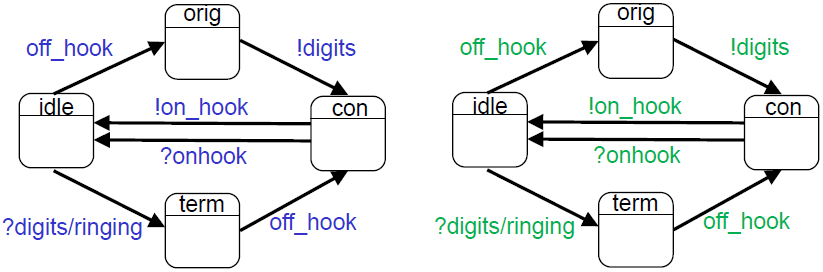
\includegraphics[width=0.8\textwidth]{pictures/phones1.png}\\
	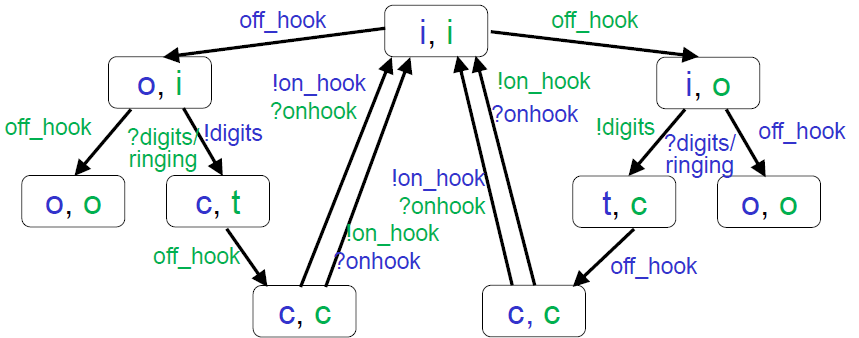
\includegraphics[width=0.8\textwidth]{pictures/phones2.png}\\
}

\card{Model Checking: Konstruktion (Berechnung) eines globalen Zustandsraums (Regeln)}{
	\begin{enumerate}
		\item Übergänge in lokalen (individuellen) Zustandsmaschinen (Statechart)
		\item Zustände im globalen Zustandsraum sind Paare der Form ($s_1,s_2$), wobei $s_1$ ein Zustand aus State Machine 1 und $s_2$ ein Zustand aus State Machine 2 ist
	\end{enumerate}
}

\card{Model Checking: Counterexample}{
	\begin{enumerate}
		\item falls eine Eigenschaftsverletzung gefunden wurde, zeigt SPIN einen Ausführungspfad vom Ausgangszustand bis zum verletzenden Zustand (hilfreich beim Debugging)
	\end{enumerate}
}

\card{Model Checking: SPIN}{
	\begin{enumerate}
		\item Syntax Check
		\item Slicing: führt eine Datenflussanalyse in Bezug auf die Eigenschaft durch, bestimmt irrelevante Teile des Modells
		\item Simulation: zufällig, interaktive oder pfadgeführte Simulation, wichtigste Debugginghilfe
		\item Verification: Model Checker, führt eine Überprüfung der Sicherheit und Lebendigkeit durch
		\item LTL Property Manager: hilft temporale Logikformeln zu bearbeiten und zu pflegen
		\item FSM View
	\end{enumerate}
}

\card{Model Checking: Never Claim}{
	\begin{enumerate}
		\item nur eine Instanz pro Promelamodell
		\item synchron mit dem Rest des Modells ausgeführt
		\item kann einen Schritt ausführen, wenn Bedinungslabel des Überganges erfüllt is im aktuellen Zustand des Promelamodells
		\item nichtdeterministischer Automat
		\item Endzustand des \textit{Never Claim} zeigt immer eine Eigenschaftsverletzung an
		\item stotternde Semantik: Endzustand wird für immer wiederholt
	\end{enumerate}
}

\card{Model Checking: Zustandsraumexplosion (Problem)}{
	\begin{enumerate}
		\item annehmen von n lokalen gleichzeitigen Prozessen (Proctypes)
		\item annehmen von K als Obergrenze für die Anzahl an Zuständen in jedem Prozess
		\item Worst Case: $K^n$
		\item Konsequenzen: Speicheranforderungen steigen exponentiell in n,\\
		Suchanstrengungen wachsen exponentiell in n\\
		Suche selbst ist Worst-Case linear
	\end{enumerate}
}

\card{Model Checking: Zustandsraumexplosion (Techniken)}{
	\begin{compactenum}
		\item On-The-Fly Search: Effizienzproblem: jeder Knoten wird zweimal besucht (Generierung der Zustände, Suche), benötigt Speicher des ganzen Zustandsraums, Gefahr: löschen von Knoten die wieder besucht werden würden; Bsp: SPIN
		\item Partial Order Reduction: reduzieren der Anzahl des erforschten\\
		Zustände und Übergänge durch Nutzung von Redundanz im Zustandsraum, Anforderungen zur Reduzierung: Eigenschaft gilt im reduzierten Zustandsraum gdw. gilt im ganzen Zustandsraum
		\item Bit-State Hashing: kein Wiederbesuchen von Zuständen $\Rightarrow$ exponentiell $\rightarrow$ linear, SPIN benutzt Hashfunktionen basierend auf Checksummenpolynomen (Jenkin's Hash), speichern eines Bits (0,1), Probleme bei Duplikaten
	\end{compactenum}
}

\card{Korrektheitsbeweis: Regeln}{
	Beweisstrategien für verschiedene Kontrollflusskonstrukte:
	\begin{enumerate}
		\item sequentielle Zusammensetzung:\\
		generelle Form: S1;S2\\
		Beweisregel:\\
		$\dfrac{\{F_1\}S_1\{F_2\},\{F_2\}S_2\{F_3\}}{\{F_1\}S_1;S_2\{F_3\}}$
		\item bedingte Aussagen (if \dots then \dots else)\\
		Beweisregel: $\dfrac{\{P \cap C\}S_1\{Q\},\{P \cap \neg C\}S_2\{Q\}}{\{P\} \text{ if C then }S_1\text{ else }S_2;\{Q\}}$
	\end{enumerate}
}
\card{Model Checking: linear temporal logic}{
	\begin{enumerate}
		\item $\square$ A: always A (immer A)
		\item $\diamond$ A: eventually A (möglicherweise A)
		\item A $\mathcal{U}$ B: A until B (A solange bis B mindestens einmal gilt)
	\end{enumerate}
}
\card{Agile Methiden}{
	\begin{enumerate}
		\item Extreme Programming
		\item Pair Programming (XP-Art)
		\item Probleme: kann schwierig sein, Interessen zu behalten, der Kunden, die im Prozess involviert sind, Verträge können ein Problem sein (wie mit anderen Ansätzen zur Durchführung)
	\end{enumerate}
}

\card{SEI Capability Maturity Model (CMM): Bild}{
	\usetikzlibrary{positioning,arrows}
\begin{tikzpicture}[node distance=0.5cm]

\node (0) at (0,0) {Initial};

\node (p0) [right=of 0,xshift=-0.25cm,yshift=-.5cm]{\phantom{jP} };
\node (p1) [above right=of p0,anchor=south,xshift=0.5cm]{\phantom{jP}};
\node (p2) [above right=of p1,anchor=south,xshift=0.5cm]{\phantom{jP}};
\node (p3) [above right=of p2,anchor=south,xshift=0.5cm]{\phantom{jP}};
\node (p4) [above right=of p3,anchor=south,xshift=0.5cm]{\phantom{jP}};
\node (p5) [above right=of p4,anchor=south,xshift=0.5cm]{\phantom{jP}};
\draw(p0.center)|-(p1.center)|-(p2.center)|-(p3.center)|-(p4.center)|-(p5.center);

\node (1) [left=of p1,yshift=.5cm]{Repeatable};
\node (2) [left=of p2,yshift=.5cm]{Defined};
\node (3) [left=of p3,yshift=.5cm]{Managed};
\node (4) [left=of p4,yshift=.5cm]{Optimizing};

\node (0) [right=of p0,yshift=.5cm,xshift=-0.5cm]{\Large 1};
\node (0) [right=of p1,yshift=.5cm,xshift=-0.5cm]{\Large 2};
\node (0) [right=of p2,yshift=.5cm,xshift=-0.5cm]{\Large 3};
\node (0) [right=of p3,yshift=.5cm,xshift=-0.5cm]{\Large 4};
\node (0) [right=of p4,yshift=.5cm,xshift=-0.5cm]{\Large 5};
\end{tikzpicture}
}
\card{SEI Capability Maturity Model (CMM): Beschreibung}{
	\begin{description}
		\item[Initial] Ad-hoc, chaotisch, heroische Programmierer
		\item[Repeatable] einige Prozessdisziplin und Tracking
		\item[Defined] Prozess ist dokumentiert und standardisiert
		\item[Managed] Qualität quantitativ gesteuert/bewertet
		\item[Optimizing] kontinuierliche Prozessverbesserung
	\end{description}
}

\end{document}